\documentclass{article}

\usepackage[utf8]{inputenc}
\usepackage{amsmath, esint}
\usepackage{wasysym}
\usepackage{qrcode}
\usepackage[colorlinks]{hyperref}
\usepackage{lmodern}
\usepackage{graphicx}
\usepackage{xcolor}
\usepackage[left=2cm, top=3cm, right=2cm]{geometry}
\usepackage{minted}
\usepackage{booktabs}
\usepackage{svg}
\usepackage{xcolor}
\definecolor{LightGray}{gray}{0.975}
\hypersetup{
  urlcolor=blue
}

\title{Databases \\ Lab 05: A still `gentle' Introduction to Intermediate SQL.}
\author{Andrés Oswaldo Calderón Romero, Ph.D.}
\date{\today}


\begin{document}

\maketitle

\section{Introduction}
In this lab, we will take a hands-on approach to explore data analysis using SQL within the context of European football leagues. Working with a rich dataset that spans multiple seasons and thousands of players and matches, you will gain practical experience designing SQL queries that summarize meaningful insights from relational data.

\section{Getting Some Data}
This time, we will work with European football leagues, specifically 11 leagues from countries such as England, France, and the Netherlands. The database contains data from the 2008 to 2016 seasons, covering more than 25,000 matches and 10,000 players.
More information about the database can be found at \url{https://www.kaggle.com/datasets/hugomathien/soccer}. The dataset we will use is a simplified version that includes only a few player attributes and no team attributes. Figure \ref{fig:erd} shows the Entity-Relationship Diagram (ERD) of the database.

Please follow these steps:

\begin{enumerate}
    \item Download the \href{https://drive.google.com/file/d/17LjylJBOfWug6y0iEgjciztVPHpv82OT/view?usp=sharing}{\texttt{euroleagues.sql}} file to an accessible location.
    \item Create a database named \textit{euroleagues}.
    \item Connect to the database.
    \item Run the command \texttt{\textbackslash{}i euroleagues.sql}. Be sure to update the path according.
    \item Enjoy!
\end{enumerate}

\begin{figure}
 \centering
 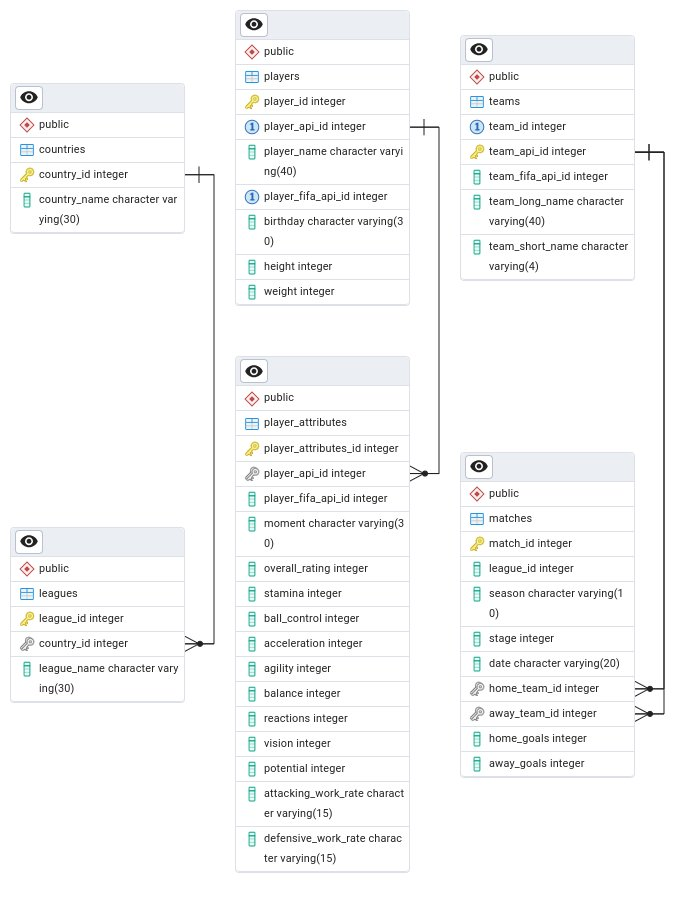
\includegraphics[width=0.8\textwidth]{figures/Euroleagues_erd.jpg}
 \caption{E-R Diagram of the Euroleagues Database.}
 \label{fig:erd}
\end{figure}

\section{SQL Sorting}

\begin{enumerate}
  \item Reorder the SQL query lines in Table~\ref{tab:messi-cristiano} to determine which player ranks higher --Messi or Cristiano Ronaldo.

  \item Reorder the SQL query lines in Table~\ref{tab:potential} to list players whose potential exceeds the global average and whose height is $\leq 170\,\mathrm{cm}$.
\end{enumerate}


\begin{table}[t]
  \centering
  \caption{Messi or Cristiano}
  \label{tab:messi-cristiano}
  \begin{tabular}{ r p{0.8\linewidth}}
    \toprule
    \textbf{Pos}
    %& \textbf{Original Pos}
    & \textbf{SQL Line} \\
    \midrule
    1
    %& 16
    & FROM stats \\
    2
    %& 10
    &   FROM candidates c \\
    3
    %& 11
    &   JOIN public.player\_attributes pa \\
    4
    %& 17
    & ORDER BY avg\_overall DESC, max\_overall DESC; \\
    5
    %& 14
    & ) \\
    6
    %& 3
    &   FROM public.players p \\
    7
    %& 4
    &   WHERE p.player\_name LIKE '\%Messi\%' OR p.player\_name LIKE '\%Cristiano R\%' \\
    8
    %& 1
    & WITH candidates AS ( \\
    9
    %& 9
    &          MAX(pa.overall\_rating) AS max\_overall \\
    10
    %& 8
    &          AVG(pa.overall\_rating) AS avg\_overall, \\
    11
    %& 2
    &   SELECT p.player\_api\_id, p.player\_name AS who \\
    12
    %& 15
    & SELECT *  \\
    13
    %& 12
    &   ON pa.player\_api\_id = c.player\_api\_id \\
    14
    %& 7
    &   SELECT c.who, \\
    15
    %& 6
    & stats AS ( \\
    16
    %& 5
    & ), \\
    17
    %& 13
    &   GROUP BY c.who \\
    \bottomrule
  \end{tabular}
\end{table}

\begin{table}[t]
  \centering
  \caption{Above potential}
  \label{tab:potential}
  \begin{tabular}{r p{0.75\linewidth}}
    \toprule
    \textbf{Pos}
    %& \textbf{Original Pos}
    & \textbf{SQL Line} \\
    \midrule
    1
    %& 10
    &   FROM A \\
    2
    %& 6
    &   GROUP BY pa.player\_api\_id, p.player\_name \\
    3
    %& 16
    & 	p.height $\leq$ 170 \\
    4
    %& 4
    &   NATURAL JOIN public.players p \\
    5
    %& 7
    & ), \\
    6
    %& 9
    &   SELECT AVG(player\_potential) AS general\_potential \\
    7
    %& 8
    & B AS ( \\
    8
    %& 13
    & FROM public.players p \\
    9
    %& 11
    & ) \\
    10
    %& 5
    &   WHERE pa.potential IS NOT NULL \\
    11
    %& 15
    & WHERE a.player\_potential $>$ b.general\_potential AND \\
    12
    %& 1
    & WITH A AS ( \\
    13
    %& 2
    &   SELECT pa.player\_api\_id, p.player\_name, AVG(pa.potential) AS player\_potential \\
    14
    %& 14
    & NATURAL JOIN A a, B b \\
    15
    %& 3
    &   FROM public.player\_attributes pa \\
    16
    %& 12
    & SELECT p.player\_name, a.player\_potential, b.general\_potential \\
    \bottomrule
  \end{tabular}
\end{table}

\section{SQL Interpretation}

For each listing in this section, provide a concise yet thorough explanation of what the \texttt{SQL} statement does—its purpose, key operations (joins, filters, aggregations), and the expected result.

\begin{enumerate}

  \item \text{ }

  \begin{minted}
[tabsize=4, obeytabs, frame=lines, framesep=2mm, baselinestretch=1.2, bgcolor=LightGray, fontsize=\scriptsize, linenos]{sql}
WITH A AS (
  SELECT home_team_id AS team_api_id
  FROM public.matches
  WHERE home_goals = 0 AND away_goals = 0
  UNION
  SELECT away_team_id
  FROM public.matches
  WHERE home_goals = 0 AND away_goals = 0
),
B AS (
  SELECT home_team_id AS team_api_id
  FROM public.matches
  WHERE (home_goals - away_goals) >= 5
  UNION
  SELECT away_team_id
  FROM public.matches
  WHERE (away_goals - home_goals) >= 5
)
SELECT
  t.team_long_name
FROM (
  SELECT team_api_id FROM A
  INTERSECT
  SELECT team_api_id FROM B) AS foo
JOIN
  public.teams t
USING
  (team_api_id);
\end{minted}

  \item \text{ }
\begin{minted}
[tabsize=4, obeytabs, frame=lines, framesep=2mm, baselinestretch=1.2, bgcolor=LightGray, fontsize=\scriptsize, linenos]{sql}
WITH marks AS (
  SELECT
    league_id, season,
    CASE WHEN home_goals = away_goals THEN 1 ELSE 0 END AS is_draw
  FROM
    public.matches
)
SELECT
  l.league_name, m.season,
  COUNT(*) AS matches,
  SUM(m.is_draw) AS draws,
  ROUND(100.0 * SUM(m.is_draw)::numeric / COUNT(*), 2) AS draw_rate
FROM
  marks m
JOIN
  public.leagues l ON l.league_id = m.league_id
GROUP BY
  l.league_name, m.season
ORDER BY
  draw_rate DESC
LIMIT
  15;
\end{minted}

\end{enumerate}

\section{What We Expect}
Just have fun.

\vspace{5mm}
Happy Hacking \includesvg[width=4mm]{figures/sunglasses}!

\end{document}

